\documentclass[a4paper, 14pt]{extarticle}

% Поля
%--------------------------------------
\usepackage{geometry}
\geometry{a4paper,tmargin=2cm,bmargin=2cm,lmargin=3cm,rmargin=1cm}
%--------------------------------------


%Russian-specific packages
%--------------------------------------
\usepackage[T2A]{fontenc}
\usepackage[utf8]{inputenc} 
\usepackage[english, main=russian]{babel}
%--------------------------------------

\usepackage{textcomp}

% Красная строка
%--------------------------------------
\usepackage{indentfirst}               
%--------------------------------------             


%Graphics
%--------------------------------------
\usepackage{graphicx}
\graphicspath{ {./images/} }
\usepackage{wrapfig}
%--------------------------------------

% Полуторный интервал
%--------------------------------------
\linespread{1.3}                    
%--------------------------------------

%Выравнивание и переносы
%--------------------------------------
% Избавляемся от переполнений
\sloppy
% Запрещаем разрыв страницы после первой строки абзаца
\clubpenalty=10000
% Запрещаем разрыв страницы после последней строки абзаца
\widowpenalty=10000
%--------------------------------------

%Списки
\usepackage{enumitem}

%Подписи
\usepackage{caption} 

%Гиперссылки
\usepackage{hyperref}

\hypersetup {
	unicode=true
}

%Рисунки
%--------------------------------------
\DeclareCaptionLabelSeparator*{emdash}{~--- }
\captionsetup[figure]{labelsep=emdash,font=onehalfspacing,position=bottom}
%--------------------------------------

\usepackage{tempora}

%Листинги
%--------------------------------------
\usepackage{listings}
\lstset{
  basicstyle=\ttfamily\footnotesize, 
  %basicstyle=\footnotesize\AnkaCoder,        % the size of the fonts that are used for the code
  breakatwhitespace=false,         % sets if automatic breaks shoulbd only happen at whitespace
  breaklines=true,                 % sets automatic line breaking
  captionpos=t,                    % sets the caption-position to bottom
  inputencoding=utf8,
  frame=single,                    % adds a frame around the code
  keepspaces=true,                 % keeps spaces in text, useful for keeping indentation of code (possibly needs columns=flexible)
  keywordstyle=\bf,       % keyword style
  numbers=left,                    % where to put the line-numbers; possible values are (none, left, right)
  numbersep=5pt,                   % how far the line-numbers are from the code
  xleftmargin=25pt,
  xrightmargin=25pt,
  showspaces=false,                % show spaces everywhere adding particular underscores; it overrides 'showstringspaces'
  showstringspaces=false,          % underline spaces within strings only
  showtabs=false,                  % show tabs within strings adding particular underscores
  stepnumber=1,                    % the step between two line-numbers. If it's 1, each line will be numbered
  tabsize=2,                       % sets default tabsize to 8 spaces
  title=\lstname                   % show the filename of files included with \lstinputlisting; also try caption instead of title
}
%--------------------------------------

%%% Математические пакеты %%%
%--------------------------------------
\usepackage{amsthm,amsfonts,amsmath,amssymb,amscd}  % Математические дополнения от AMS
\usepackage{mathtools}                              % Добавляет окружение multlined
\usepackage[perpage]{footmisc}
%--------------------------------------

%--------------------------------------
%			НАЧАЛО ДОКУМЕНТА
%--------------------------------------

\begin{document}

%--------------------------------------
%			ТИТУЛЬНЫЙ ЛИСТ
%--------------------------------------
\begin{titlepage}
\thispagestyle{empty}
\newpage


%Шапка титульного листа
%--------------------------------------
\vspace*{-60pt}
\hspace{-65pt}
\begin{minipage}{0.3\textwidth}
\hspace*{-20pt}\centering

\includegraphics[width=\textwidth]{emblem}
\end{minipage}
\begin{minipage}{0.67\textwidth}\small \textbf{
\vspace*{-0.7ex}
\hspace*{-6pt}\centerline{Министерство науки и высшего образования Российской Федерации}
\vspace*{-0.7ex}
\centerline{Федеральное государственное бюджетное образовательное учреждение }
\vspace*{-0.7ex}
\centerline{высшего образования}
\vspace*{-0.7ex}
\centerline{<<Московский государственный технический университет}
\vspace*{-0.7ex}
\centerline{имени Н.Э. Баумана}
\vspace*{-0.7ex}
\centerline{(национальный исследовательский университет)>>}
\vspace*{-0.7ex}
\centerline{(МГТУ им. Н.Э. Баумана)}}
\end{minipage}
%--------------------------------------

%Полосы
%--------------------------------------
\vspace{-25pt}
\hspace{-35pt}\rule{\textwidth}{2.3pt}

\vspace*{-20.3pt}
\hspace{-35pt}\rule{\textwidth}{0.4pt}
%--------------------------------------

\vspace{1.5ex}
\hspace{-35pt} \noindent \small ФАКУЛЬТЕТ\hspace{30pt} <<Информатика, искусственный интеллект и системы управления>>

\vspace*{-16pt}
\hspace{47pt}\rule{0.83\textwidth}{0.4pt}

\vspace{0.5ex}
\hspace{-35pt} \noindent \small КАФЕДРА\hspace{50pt} <<Теоретическая информатика и компьютерные технологии>>

\vspace*{-16pt}
\hspace{30pt}\rule{0.866\textwidth}{0.4pt}
  
\vspace{11em}

\begin{center}
\Large {\bf Лабораторная работа № 2} \\ 
\large {\bf по курсу <<Языки и методы программирования>>} \\
\large <<Разработка простейшего класса на языке Java>> 
\end{center}\normalsize

\vspace{8em}


\begin{flushright}
  {Студент группы ИУ9-21Б Яннаев А. С. \hspace*{15pt}\\ 
  \vspace{2ex}
  Преподаватель Посевин Д. П.\hspace*{15pt}}
\end{flushright}

\bigskip

\vfill
 

\begin{center}
\textsl{Москва 2025}
\end{center}
\end{titlepage}
%--------------------------------------
%		КОНЕЦ ТИТУЛЬНОГО ЛИСТА
%--------------------------------------

\renewcommand{\ttdefault}{pcr}

\setlength{\tabcolsep}{3pt}
\newpage
\setcounter{page}{2}

\section{Задание}\label{Sect::task}
\begin{enumerate}
\item Выполнение лабораторной работы заключается в составлении на языке Java одного из
классов, приведённых в таблице. В классе обязательно должны присутствовать конструктор и метод toString.


\item Отладку разработанного класса необходимо осуществить в методе main
вспомогательного класса Test. Использование контейнерных классов из стандартной библиотеки языка Java не разрешается.

\item Класс стреловидных матриц размера n n с операцией вычисления определителя. Все элементы стреловидной матрицы, кроме принадлежащих первой строке, первому столбцу или главной диагонали, равны нулю. Матрица должна быть представлена в виде, исключающем хранение заведомо нулевых элементов.


\end{enumerate}
\section{Результаты}\label{Sect::res}

Исходный код программы представлен в ~\ref{lst:code1}, ~\ref{lst:code2}.
Результат запуска представлен на рисунке ~\ref{fig:img1}, ~\ref{fig:img2}.

\begin{figure}[!htb]
\begin{lstlisting}[language={java},caption={Файл ArrowMatrix.java},label={lst:code1}]
public class ArrowMatrix {
    private int n;
    private double[][] matrix;
    public ArrowMatrix(int n, double[] firstRow, double[] firstColumn, double[] mainDiagonal) {
        this.n = n;
        this.matrix = new double[n][n];
        for (int i = 0; i < n; i++) {
            matrix[0][i] = firstRow[i];
            matrix[i][0] = firstColumn[i];
            if (i > 0) { matrix[i][i] = mainDiagonal[i]; }
        }
    }
    public double determinant() {
        return computeDeterminant(matrix, n);}
    private double computeDeterminant(double[][] mat, int size) {
        if (size == 1) { return mat[0][0]; }
        if (size == 2) { return mat[0][0] * mat[1][1] - mat[0][1] * mat[1][0]; }
        double det = 0;
        for (int i = 0; i < size; i++) {
            double[][] subMatrix = getSubMatrix(mat, size, i);
            double cofactor = (i % 2 == 0 ? 1 : -1) * mat[0][i] * computeDeterminant(subMatrix, size - 1);
            det += cofactor;
        }
        return det;
    }
    private double[][] getSubMatrix(double[][] mat, int size, int column) {
        double[][] subMatrix = new double[size - 1][size - 1];
        for (int i = 1; i < size; i++) {
            int subCol = 0;
            for (int j = 0; j < size; j++) {
                if (j == column) continue;
                subMatrix[i - 1][subCol] = mat[i][j];
                subCol++;
            }
        }
        return subMatrix;
    }
    public String toString() {
        StringBuilder result = new StringBuilder();
        for (int i = 0; i < n; i++) {
            for (int j = 0; j < n; j++) {
                result.append(String.format("%10.1f ", matrix[i][j]));
            }
            result.append("\n");
        }
        return result.toString();
    }
}



\end{lstlisting}
\end{figure}

\begin{figure}[!htb]
\begin{lstlisting}[language={java},caption={Файл Test.java},label={lst:code2}]
import java.util.Scanner;
public class Test {
    public static void main(String[] args) {
        Scanner scanner = new Scanner(System.in);
        int n;
        while (true) {
            System.out.print("size (n): ");
            n = scanner.nextInt();
            if (n > 0) break;
            System.out.println("size > 0.");
        }
        double[] firstRow = new double[n];
        double[] firstColumn = new double[n];
        double[] mainDiagonal = new double[n];
        while (true) {
            System.out.println("\n1st row:");
            for (int i = 0; i < n; i++) {
                System.out.print("firstRow[" + i + "]: ");
                firstRow[i] = scanner.nextDouble();
            }
            System.out.println("\1st column:");
            for (int i = 0; i < n; i++) {
                System.out.print("firstColumn[" + i + "]: ");
                firstColumn[i] = scanner.nextDouble();
            }
            System.out.println("\main diag:");
            for (int i = 1; i < n; i++) {
                System.out.print("mainDiagonal[" + i + "]: ");
                mainDiagonal[i] = scanner.nextDouble();
            }
            ArrowMatrix matrix = new ArrowMatrix(n, firstRow, firstColumn, mainDiagonal);
            System.out.println("\matrix:");
            System.out.println(matrix);
            System.out.print("right?: ");
            String answer = scanner.next();
            if (answer.equals("yes")) {
                System.out.println("\det: " + matrix.determinant());
                break;
            }
            System.out.println("try again");
        }
        scanner.close();
    }
}


\end{lstlisting}
\end{figure}


\begin{figure}[!htb]
	\centering
	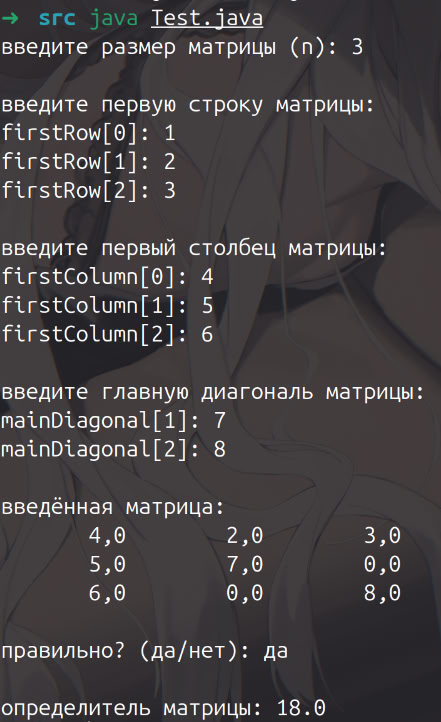
\includegraphics[width=0.8\textwidth]{img2}
\caption{Результат вывода в консоли}
\label{fig:img1}
\end{figure}

\begin{figure}[!htb]
	\centering
	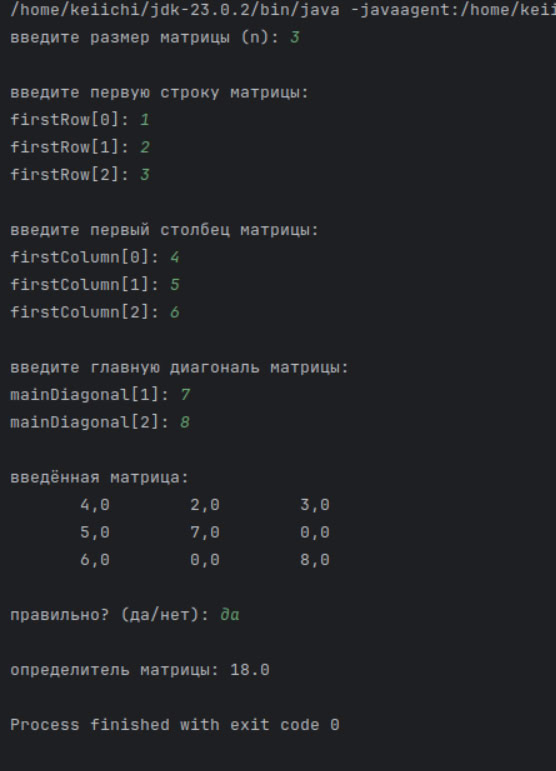
\includegraphics[width=0.8\textwidth]{img1}
\caption{Результат вывода в  IntelliJ IDEA}
\label{fig:img2}
\end{figure}

\end{document}
